\documentclass[a4paper,12pt]{article}
\usepackage[utf8]{inputenc} % Codificação UTF-8
\usepackage[T1]{fontenc}    % Suporte para caracteres acentuados
\usepackage{amsmath, amssymb} % Pacotes para fórmulas matemáticas
\usepackage{graphicx}        % Inclusão de gráficos
\usepackage{pgfplots}        % Criação de gráficos no LaTeX
\usepackage{hyperref}        % Links e referências

\title{Introdução às Séries de Fourier}
\author{}
\date{}

\begin{document}

\maketitle

\section*{Definição da Série de Fourier}
As séries de Fourier permitem representar funções periódicas como uma soma infinita de funções senoidais (senos e cossenos). Seja $f(x)$ uma função periódica de período $T$, a série de Fourier é dada por:
\[
f(x) = a_0 + \sum_{n=1}^\infty \left[ a_n \cos\left(\frac{2\pi n x}{T}\right) + b_n \sin\left(\frac{2\pi n x}{T}\right) \right],
\]
onde:
\[
a_0 = \frac{1}{T} \int_{0}^{T} f(x) \, dx,
\]
\[
a_n = \frac{2}{T} \int_{0}^{T} f(x) \cos\left(\frac{2\pi n x}{T}\right) dx,
\]
\[
b_n = \frac{2}{T} \int_{0}^{T} f(x) \sin\left(\frac{2\pi n x}{T}\right) dx.
\]

Os coeficientes $a_n$ e $b_n$ determinam a contribuição de cada componente senoidal para a reconstrução de $f(x)$.

\section*{Exemplo Clássico: Onda Quadrada}
Consideremos a função onda quadrada $f(x)$, definida no intervalo $[-\pi, \pi]$:
\[
f(x) = 
\begin{cases} 
1, & -\pi \leq x < 0, \\
-1, & 0 \leq x \leq \pi.
\end{cases}
\]
Esta função pode ser representada pela série de Fourier:
\[
f(x) = \sum_{n=1, \text{ ímpar}}^\infty \frac{4}{n\pi} \sin(nx).
\]

\section*{Gráfico da Onda Quadrada e Aproximação por Fourier}
Abaixo, apresentamos o gráfico da onda quadrada e sua aproximação usando os primeiros 5 termos da série de Fourier.

\begin{figure}[h!]
\centering
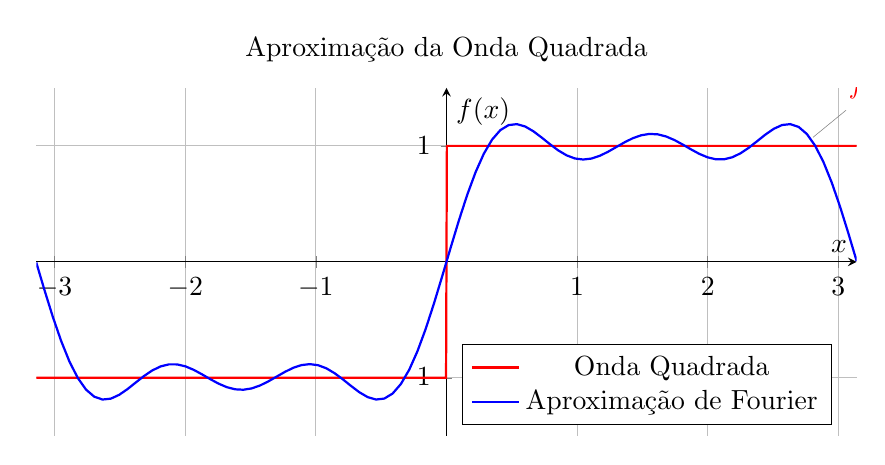
\begin{tikzpicture}
\begin{axis}[
    domain=-3.14:3.14, 
    samples=1000, 
    xlabel={$x$}, ylabel={$f(x)$}, 
    legend pos=south east,
    axis lines=middle, 
    width=12cm, height=6cm, 
    ymin=-1.5, ymax=1.5, 
    grid=major, 
    title={Aproximação da Onda Quadrada}
]
    \addplot[thick, red, domain=-3.14:3.14] {sign(sin(deg(x)))} node[pos=0.95,pin=45:{$f(x)$}] {};
    \addplot[blue, thick, samples=100, domain=-3.14:3.14]
    {4/pi*(sin(deg(x)) + 1/3*sin(3*deg(x)) + 1/5*sin(5*deg(x)))}; 
    \legend{Onda Quadrada, Aproximação de Fourier}
\end{axis}
\end{tikzpicture}
\caption{Reconstrução da onda quadrada usando 5 termos da série de Fourier.}
\end{figure}

\section*{Conclusão}
A série de Fourier aproxima a função original ao somar termos senoidais de diferentes frequências. Quanto mais termos incluímos, mais próxima a reconstrução se torna, com exceção de pontos de descontinuidade, onde ocorre o \emph{fenômeno de Gibbs}.

\end{document}
